\documentclass[toc=bibliography,openany, twoside, abstracton]{scrartcl}


%%% File encoding is ISO-8859-1 (also known as Latin-1)
%%% You can use special characters just like ä,ü and ñ

% Input encoding is 'latin1' (Latin 1 - also known as ISO-8859-1)
% CTAN: http://www.ctan.org/pkg/inputenc
%
% A newer package is available - you may look into:
% \usepackage[x-iso-8859-1]{inputenc}
% CTAN: http://www.ctan.org/pkg/inputenx
\usepackage[utf8]{inputenc}
\usepackage{import}
\usepackage{dsfont}
% Font Encoding is 'T1' -- important for special characters such as Umlaute ü or ä and special characters like ñ (enje)
% CTAN: http://www.ctan.org/pkg/fontenc
\usepackage[T1]{fontenc}
%\usepackage[osf, sc]{mathpazo} % Use the Palatino font

% Language support for 'english' (alternatives: british,UKenglish,USenglish,american)
% CTAN: http://www.ctan.org/pkg/babel
\usepackage[english]{babel} %
\usepackage{csquotes}

% Extended graphics support
% There is also a package named 'graphics' - watch out!
% CTAN: http://www.ctan.org/pkg/graphicx
\usepackage{graphicx}

%customized line spacing
\usepackage{setspace}
\usepackage{dirtytalk}
%Inclusion of pdf's
\usepackage{pdfpages}

%Create random text
\usepackage{lipsum} % \lipsum[1] or \lipsum[1-3]

% biblatex is used for creating bibliography
\usepackage[style=authoryear, backend=bibtex8, natbib=true, maxcitenames=2]{biblatex}

% More comprehensive math typing
\usepackage{amssymb}

% To allow new math operators
\usepackage{amsmath}
\usepackage{mathtools}
\usepackage{bm} % bold symbol in math mode

% Nice matrix features
\usepackage{physics}
\usepackage[ruled,vlined]{algorithm2e}
% Abbreviations
\usepackage[hyperref=true]{acro}

% Structure
\usepackage{float}
\usepackage{placeins}
\usepackage{multirow}
\usepackage{multicol}
\usepackage{pdfpages}
\usepackage{kbordermatrix}% http://www.hss.caltech.edu/~kcb/TeX/kbordermatrix.sty

% Tables, figures
\usepackage{booktabs} %Create publication quality tables
\usepackage{tabularx}
\usepackage{threeparttable}
\usepackage{siunitx}
\usepackage[figuresright]{rotating}
\usepackage{subcaption}
\usepackage{caption}
\newcommand{\sourcecenter}[1]{\vspace{-6pt} \caption*{\textit{Source: } { #1} \hfill} } % centered
\newcommand{\sourceleft}[1]{\vspace{-18pt} \caption*{\textit{Source: } { #1} \hspace*{\fill}} }  % left-aligned

% Text
\usepackage{xcolor}
\usepackage{enumerate} % numbered lists
\usepackage[super]{nth} % Write 1st, 2nd as \nth{1}, \nth{2} etc.
\usepackage{listings} % see https://tex.stackexchange.com/questions/105662/default-value-for-basicstyle-in-lstlisting

% Front page
%Add affiliations to authors name, allowing to mix affiliations
\usepackage{authblk}  % \author[a]{F. Hvam} \author[a]{S. Tarly} \author[b]{J. Snow}
                      % \affil[a]{The Citadel} \affil[b]{The Wall}
\newenvironment{acknowledgements}{ %acknowledgements for title page
  \renewcommand\abstractname{Acknowledgements}\begin{abstract}} {\end{abstract}}

% Notes
\usepackage{epigraph}
\usepackage{marginnote}
% Select what to do with command \comment:
  % \newcommand{\comment}[1]{}  %comments not showed
   \newcommand{\comment}[1]{\par {\bfseries \color{blue} #1 \par}} %comments showed
% Select what to do with todonotes: i.e. \todo{}, \todo[inline]{}
  %\usepackage[disable]{todonotes} % notes not showed
   \usepackage[draft]{todonotes}   % notes showed

% % 'Ditto' signs for tables
% \usepackage{tikz}
%   \newcommand{\ditto}{
%       \tikz{
%           \draw [line width=0.12ex] (-0.2ex,0) -- +(0,0.8ex)
%               (0.2ex,0) -- +(0,0.8ex);
%           \draw [line width=0.08ex] (-0.6ex,0.4ex) -- +(-1.0em,0)
%               (0.6ex,0.4ex) -- +(1.0em,0);
%       }
%   }


%%% File encoding is ISO-8859-1 (also known as Latin-1)
%%% You can use special characters just like ä,ü and ñ

% Special KOMA-Script package - I added it because I also use the float package in this template, see:
% http://tex.stackexchange.com/questions/51867/koma-warning-about-toc
% CTAN: http://www.ctan.org/tex-archive/macros/latex/contrib/koma-script/doc
\usepackage{scrhack}

% Better support for marginnotes
% new command: \marginnote
% LaTeX standard command: \marginpar
% CTAN: http://www.ctan.org/pkg/marginnote
\usepackage{marginnote}

% Extended header and footer support
% CTAN: http://www.ctan.org/pkg/scrpage2
\usepackage[%
  	automark
  	,ilines
	,headsepline
	,footsepline
]{scrpage2}



\newcommand\crule[3][black]{\textcolor{#1}{\rule{#2}{#3}}}

% what ages of childen do we accept
\newcommand{\minage}{10}
\newcommand{\maxage}{15}

% safetime end
\newcommand{\safeend}{1990}

\newcommand{\safelength}{4}   % saveend - 1987 + 1

% when is the event window open?
\newcommand{\winstart}{1991}
\newcommand{\winend}{1993}


%%% File encoding is ISO-8859-1 (also known as Latin-1)
%%% You can use special characters just like ä,ü and ñ

% User friendly interface to change layout parameters
% CTAN: http://www.ctan.org/pkg/geometry
\usepackage{geometry}
\geometry{% siehe geometry.pdf (Figure 1)
	bottom=30mm,
	showframe=false, % For debugging: try true and see the layout frames
	margin=30mm,
	marginparsep=3mm,
	marginparwidth=20mm
}


% The file include userdefined colours

\definecolor[named]{myColorMainA}{RGB}{0,0,0}
\definecolor[named]{myColorMainB}{RGB}{0,0,0}

\definecolor[named]{darkgreen}{HTML}{008000}


%%% File encoding is ISO-8859-1 (also known as Latin-1)
%%% You can use special characters just like ä,ü and ñ

% ##############################################
% Start: Table of Contents (TOC) Customization
% ##############################################
%

% Level for numbered captions
\setcounter{secnumdepth}{5}

% Level of chapters that appear in Table of Contents
\setcounter{tocdepth}{5} % bis wohin ins Inhaltsverzeichnis aufnehmen
% -2 no caption at all
% -1 part
% 0  chapter
% 1  section
% 2  subsection
% 3  subsubsection
% 4  paragraph
% 5  subparagraph

% KOMA-Script code to adjust TOC
% Applying the color 'myColorMainA' which is defined in the main file (MainFile.tex)
%\makeatletter
%\addtokomafont{chapterentrypagenumber}{\color{myColorMainA}}
%\addtokomafont{chapterentry}{\color{myColorMainA}}
%\makeatother

%
% #######################
% End: Table of Contents (TOC) Customization
% #######################

% ##############################################
% Start: Floating Object Customization
% ##############################################
%

% Extended support for catioons of figures and tables etc.
% CTAN: http://www.ctan.org/pkg/caption
\usepackage[%
	font={small},
	labelfont={bf,sf},
	format=hang, % try plain or hang
	margin=5pt,
]{caption}
%

% #######################
% End: Floating Object Customization
% #######################

% ##############################################
% Start: Headings Customization
% ##############################################
%

% KOMA-Script code to customize the headings
% Applying the color 'myColorMainA' which is defined in the main file (MainFile.tex)
%\addtokomafont{chapter}{\color{myColorMainA}}
%\addtokomafont{section}{\color{myColorMainA}}
%\addtokomafont{subsection}{\color{myColorMainA}}
%\addtokomafont{subsubsection}{\color{myColorMainA}}
%\addtokomafont{paragraph}{\color{myColorMainA}}
%\addtokomafont{subparagraph}{\color{myColorMainA}}



% Here we adjust the various section titles
\setkomafont{title}{\normalfont\Huge\bfseries}
\setkomafont{section}{\normalfont\Large\centering\scshape}
\setkomafont{subsection}{\normalfont\large\bfseries}
\setkomafont{subsubsection}{\normalfont\bfseries}
\setkomafont{paragraph}{\normalfont\bfseries}
\setkomafont{subparagraph}{\normalfont\bfseries}
\setkomafont{sectionentry}{\normalfont\bfseries}
% #######################
% End: Headings Customization
% #######################


% ##############################################
% Start: Header and Footer Customization
% ##############################################
%

% KOMA-Script code for header and footer font
\setkomafont{pageheadfoot}{%
	\normalfont\bfseries
	}
\setkomafont{pagefoot}{%
	\normalfont
	}
\setkomafont{pagenumber}{%
	\normalfont
	}

% Define width of header
\setheadwidth[0pt]{textwithmarginpar}

% Define with of header line
\setheadsepline{0.4pt}

% Define width of footer
\setfootwidth[0pt]{text}
% Define with of footer line (here: no line)
\setfootsepline[text]{0pt}

% Some calculations
% calc package is needed which is loaded here: 01_Preamble/CommonPackages.tex
% If you want to understand the calculations visit:
% http://en.wikibooks.org/wiki/LaTeX/Page_Layout
\newlength{\myLenghthFootAbstand}
\setlength{\myLenghthFootAbstand}{\paperheight-1in-\topmargin- \headheight-\headsep-\textheight-\footskip}
\newlength{\myLenghthTemp}
\setlength{\myLenghthTemp}{\myLenghthFootAbstand+\baselineskip}

% Define content of header and footer
% Using some scrpage2 commands here. The scrpage2 package is loaded here: 01_Preamble/KOMA-Script-Packages.tex
% Some LaTeX magic...
% Clear all defaults
\clearscrheadfoot
% Header
\ohead{%
	\textcolor{myColorMainA}{\headmark}
	}
% Left (even page numbers) footer
\lefoot%
[% scrplain style (begin)
	\setlength{\unitlength}{\myLenghthFootAbstand}%
	\begin{picture}(0,0)%
		\put(0,-1)%
		{%
			\makebox(0,0)[lb]%
			{%
				\rule{0.4pt}{\myLenghthTemp}%
			}%
		}%
	\end{picture}\llap{\pagemark~}%
]% scrplain style (end)
%
{% scrheadings style (begin)
	\setlength{\unitlength}{\myLenghthFootAbstand}%
	\begin{picture}(0,0)%
		\put(0,-1)%
		{%
			\makebox(0,0)[lb]%
			{%
				\rule{0.4pt}{\myLenghthTemp}%
			}%
		}%
	\end{picture}\llap{\pagemark~}%
}% scrheadings style (end)

% Right (odd page numbers) footer
\rofoot%
[% scrplain style (begin)
	\rlap{~\pagemark}%%
	\setlength{\unitlength}{\myLenghthFootAbstand}%
	\begin{picture}(0,0)%
		\put(0,-1)%
		{%
			\makebox(0,0)[lb]%
			{%
				\rule{0.4pt}{\myLenghthTemp}%
			}%
		}%
	\end{picture}%
]% scrplain style (end)
%
{% scrplain style (begin)
	\rlap{~\pagemark}%%
	\setlength{\unitlength}{\myLenghthFootAbstand}%
	\begin{picture}(0,0)%
		\put(0,-1)%
		{%
			\makebox(0,0)[lb]%
			{%
				\rule{0.4pt}{\myLenghthTemp}%
			}%
		}%
	\end{picture}%
}% scrplain style (end)

%
% #######################
% End: Header and Footer Customization
% #######################


%%% File encoding is ISO-8859-1 (also known as Latin-1)
%%% You can use special characters just like ä,ü and ñ

% This is an suggestion from Axel Reichert (LaTeX package author)
% See CTAN: http://www.ctan.org/author/reichert
% See CTAN: http://www.ctan.org/pkg/l2tabu-english (Cgapter: 1.8 Should I use \sloppy?)

\tolerance 1414
\hbadness 1414
\emergencystretch 1.5em
\hfuzz 0.3pt
\widowpenalty=10000
\vfuzz \hfuzz
\raggedbottom


%%% File encoding is ISO-8859-1 (also known as Latin-1)
%%% You can use special characters just like ä,ü and ñ

% Package for PDF features such as bookmarks and hyperlinks.
% Important: Should be loaded at the end.
% CTAN: http://www.ctan.org/pkg/hyperref
\usepackage[%
bookmarks, % Create bookmarks
bookmarksopen=true, % Unfold bookmatk tree in PDF viewer when document is opened
bookmarksopenlevel=1, % Level of unfolding
bookmarksnumbered=true, % Number bookmarks
hidelinks, % do not highlight hyperlinks -- looks ugly
pdfpagelabels=true, % See manual...
plainpages=false, % See manual...
hyperfootnotes=true, % Hyperlinks for footnotes
hyperindex=true,
colorlinks=true,
linkcolor=black,
linktoc=all,
urlcolor = myColorMainB,
citecolor=myColorMainB % Indexeinträage verweisen auf Text
]{hyperref}


\DeclareMathOperator*{\argmin}{\arg\min\ }
\DeclareMathOperator*{\plim}{\textrm{plim}\ }


\titlehead{
% \raggedright \Large University of Copenhagen \\
% \large Department of Economics \\
\raggedleft 
\includegraphics[width=0.2 \textwidth]{03_figures/logo}}
\title{\Huge Prices in Air Transport\thanks{Access our Jupyter notebooks at \url{https://github.com/Morten-Esketveit/TSDS-gruppe-2019}} % Article title
\\ \Large Can Airport Network Characteristics Aid in Prediction? % Article subtitle
%\thanks{We are thankful to Andreas Bjerre-Nielsen, Ulf Aslak Jensen, Snorre Ralund, and Kristian Urup Larsen for their teaching of the course Topics in Social Datascience (see \href{https://github.com/abjer/tsds}{github.com/abjer/tsds}).
%We would especially like to thank Kristian Urup Larsen for his helpful feedback.
%All errors remain our own.}}
}
\author[a]{Thor Donsby Noe}
\author[a]{Morten Esketveit Rasmussen}
%\thanks{ Corresponding author. % Meaningful in case of more than one author
%\textit{E-mail:} \href{mailto:mortenpolit@gmail.com}{mortenpolit@gmail.com} (Morten E. Rasmussen).}
\author[a]{Christian Lund Sørensen}
\affil[a]{\footnotesize University of Copenhagen, Department of Economics, Denmark}

\date{\normalsize \today % Leave empty to omit a date
%\\ Preliminary version
  }
\publishers{\vspace{1cm}%
    \normalfont\normalsize%
    \parbox{\linewidth}{%
        \begin{abstract}\noindent
In this paper, we investigate whether network-related features of airports can add predictive power to a model predicting flight prices. We analyze the US air transport sector as a network with airports as nodes, and direct flights as edges. We find that the network is scale-free with a small subset of airports functioning as hubs in the network, and we produce a geographical map of the network with airports in their actual locations in the continental US. Secondly, we find that while the network has changed substantially over the last two decades, the hub-and-spoke nature of the network has remained, and individual airport centrality has been relatively stable. Thirdly, we find that the network is vulnerable to a removal of the airports acting as hubs, but fairly tolerant to removal of random nodes. Finally, we create a linear prediction model for flight prices to investigate whether network-related airport characteristics improve the predictive power in such a model. We employ elastic net regularization, and use K-fold cross-validation to determine the optimal hyper-parameters. We find that these features can be said to improve the prediction model only marginally, if at all.
\\
\\ \noindent
%\textbf{Keywords:}  {\textbullet}  {\textbullet}  {\textbullet}  {\textbullet} 
% \\ \\
% \textbf{Keystrokes:} 71.886 \textbf{Standard pages:} 30. \textbf{Contributions:} Thor Donsby Noe: 3.1, 3.2, 4.3, 4.4, 5.1, 5.2, 6.3, 7.1
\end{abstract}

    }
}


%\input{abbreviations}

\newcommand{\Aref}[1]{\hyperref[#1]{Appendix~\ref{#1}}}
\newcommand{\aref}[1]{\hyperref[#1]{appendix~\ref{#1}}}
\newcommand{\Sref}[1]{\hyperref[#1]{Section~\ref{#1}}}
\newcommand{\sref}[1]{\hyperref[#1]{section~\ref{#1}}}
\newcommand{\Tref}[1]{\hyperref[#1]{Table~\ref{#1}}}
\newcommand{\tref}[1]{\hyperref[#1]{table~\ref{#1}}}
\newcommand{\Fref}[1]{\hyperref[#1]{Figure~\ref{#1}}}
\newcommand{\fref}[1]{\hyperref[#1]{figure~\ref{#1}}}


\addbibresource{bibliography.bib}

\numberwithin{equation}{section}

\begin{document}
\setstretch{1.2}

\maketitle

\thispagestyle{empty}

\clearpage

\pagestyle{scrheadings}

\small {
% \tableofcontents
% \listoffigures
% \listoftables
% \clearpage
% \printacronyms[include-classes=abbrev,name=Abbreviations, heading=chapter*]
}
\clearpage
\normalsize

\section{Introduction}
\label{sec:intro}
% Idea: How would a geographically confined natural disaster affect the network (e.g. if it was in Atlanta?). 
% Transmission of delays?

% Motivation of the study: why you focus on this particular issue
% Hypothesis and objective(s)
% Description of the background (theoretical and empirical) that lead you to propose the hypothesis
% Approach and summary of results: what is your strategy to check the hypothesis and the main result
% Structure of the paper
Firstly we characterize the air transport sector as a network, with airports as nodes and flights as edges. Secondly, we combine results from this network-analysis with spatial and other data and attempt to predict prices on flights.


\section{Literature review}
\label{sec:background}

\subsection{US airline deregulation}
\label{subsec:b_deregulation}
The classic air transport network through most of the \nth{20} century consisted of simple point-to-point connections directly linking a small number of mayor cities as there were a relatively few number of flights overall \citep{marti2015efficiency}. Delta Airlines had established their headquarter in Atlanta which became the busiest in the US as early as 1957\footnote{\href{https://web.archive.org/web/20110301150527/http://www.atlanta-airport.com/Airport/ATL/Airport_History.aspx}{atlanta-airport.com/Airport/ATL/Airport_History.aspx}}, nonetheless, flying cross-country was still a complicated affair and it was not until the US Airline Deregulation Act of 1978 when cross-state competition was opened up and drastic changes came to the structure of the aviation industry \citep{forbes2007role, daraban2012low}. Shortly after, the hub-and-spoke structure evolved both as a business model for the individual airlines and in cooperation with regional airlines \citep{forbes2007role} as a way of increasing the frequency and coverage. Furthermore, hub-and-spoke introduced economies of scale where administration and service was less important at the spokes as as most flights frequently pass through mayor hubs.
\par
In contrast, Low Cost Carriers (LCC) emerged as well, offering point-to-point flights to secondary airports, often aiming to avoid transfers and expensive hubs \citep{daraban2012low}.

\subsection{Fare determination}
\label{subsec:b_fare}
The determinants of fares (flight prices) is investigated in a number of academic papers. In \citet{vowles2006airfare}, the author states that research has focused on three areas: The role of hub and spoke networks, airfare pricing determinants, and the role of LCC. In the aforementioned paper, the author investigates fare determinants in hub-to-hub markets. He finds, that the number of passengers, distance between airports, the share of low cost carriers, the presence of multiple airports in the geographical region and the presence of Southwest Airlines in the market or competing markets all have statistically significant effects on fares.
\par
\citet{brueckner2001model} presents a theoretical model of fare and frequency determination, and compares outcomes in a hub-and-spoke network to outcomes in a fully connected network. They find, that the hub-and-spoke network yields higher flight frequency, and higher prices for passengers whose origin or ultimate destination is a hub. The explanation for the somewhat surprising latter result is that higher frequency allows airlines to extract a higher fare from passengers in spite of lower costs.
\par
\citet{abda2012impacts} examines the impact of low cost carriers on fares in the United States. They find statistically significant effects of low cost carriers (entry or substantial growth) on flight prices.  
\medskip\\
Another obvious price determinant is distance travelled through forgone time and fuel burn. In this aspect hub-and-spoke networks are far less efficient than point-to-point flights due to transferring being both time- and fuel consuming with an extra set of landing, taxiing, waiting, and take-off as compared to cruising directly. While aviation fuel is exempted from taxes for now, simulating network construction given a carbon tax result in a higher share of direct point-to-point flights relative to transfers and stop-overs \citep{o2012fuel}.

\subsection{Modelling Airport Networks}
\citet[pp. 41-42]{costa2011analyzing} provides a brief overview on the literature of networks in the context of airports including important findings and methodology. In this literature airports are defined as nodes, and flights as edges. Typically these networks are treated as directed although most flights are back and forth between two cities. Among the highlighted findings is that the degree distribution of airport networks seem to follow the power law (this is the case for studies of the whole World, India, Brazil, and the US) which in short means that the networks are characterized by a few large hubs with a much higher degree than the average airport.\footnote{Contrary to this, \citet{he2004statistics} finds that the Chinese network of airports does not follow the power law.} It is further suggested that the topology of the network is primarily determined by GDP and population size across cities in the network.
\medskip\\
\citet{chi2004structural} show the US airport network is affected by "errors" and "attacks". Their dataset covers 215 US airports, and flights in a specific week. To simulate an attack, they successively remove airports in order of importance, starting with the most connected airport. Conversely, to simulate an error, the authors remove airports in order of fewest connections. They then investigate how errors and attacks respectively influence key topological measures, specifically the average degree, the clustering coefficient, the diameter and efficiency. They find, that these measures are affected far more by removal of the most well connected airports, compared to removal of the least connected airports.
\medskip\\
\citet{rocha2017dynamics} outlines the fundamental properties of airport networks and surveys the literature on the dynamic modelling of these networks. He divides the research on dynamic modelling into two categories one in which long-term structural changes are analyzed using network ``snapshots'' and one that focuses on short-term changes which is used to analyze how delays propagate through the network and the logistics of the airport industry. Considering the first category, the literature mainly focuses on changes in basic network statistics over time. First, it is described how the deregulation of the American transportation sector changed the airport network from point-to-point to hub-and-spoke systems. Even though the airport networks have changed continually since then, the degree distribution seems to be quite constant. On the other hand, betweenness centrality and the clustering structure of the network seems to change over time.
\par
Looking at the short-term dynamics, it is found that airports that may be close in the static network can be quite far away from each other in a dynamic network since some routes are operated very infrequently.  




\section{Theory}
\label{sec:theory}
% Theoretical arguments in the literature closely related to your study

\subsection{Airline business models}
As outlined in the background in section \ref{subsec:b_deregulation} The common trend is that airlines specialize in either of two mayor business models with very different network characteristics.

\subsubsection{Point-to-point network}


\subsubsection{Hub-and-spoke network}
The
A hub-and-spoke network




\begin{figure}[H]
  \centering
  \caption{Point-to-point network (Panel a) vs hub-and-spoke network (Panel b)}
    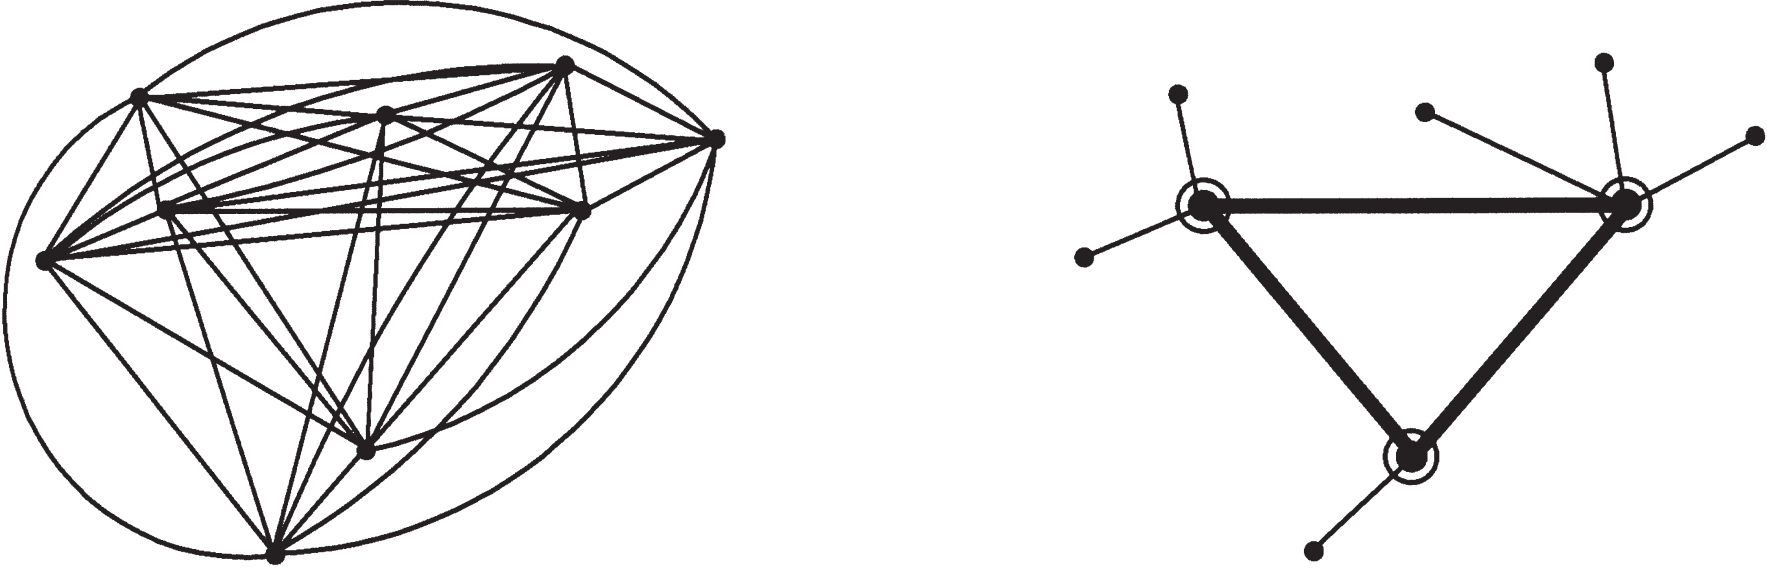
\includegraphics[width=1. \textwidth]{03_figures/Bryan_1999_networks}
    \sourcecenter{\citet{bryan1999hub}}
  \label{fig:Bryan1999}
\end{figure}



\subsection{Network Theory}
\label{subsec:Network Theory}
<<<<<<< HEAD
We draw on network theory to characterize how airports are connected to each other, what role the individual airport plays
=======
We draw on network theory to characterize how airports are connected to each other and analyze what role the individual airport plays in the network of airports. The ultimate aim of this analysis is to assess whether flight prices between airports depend on the role each airport plays in the network. \\
We view airports as nodes in the n

>>>>>>> f456b818a2fb556eea1ca8e72fb081a424cd5779


%Notes:


\section{Data and scraping}
\label{sec:data}
% Main characteristics of the data set: source, type of data
% Description of variables used for the	analysis and correspondence with the (ideal) magnitudes in the empirical specification
% Descriptive statistics of the	main variables in the analysis
Data for the analysis comes from a variety of sources.
In general, we have three types of data:
\begin{itemize}
    \item Airports. Data on airports. In the network setting, these correspond to nodes in the network.
    \item Flights/connections. These datasets contain information on flights or connections between airports. As will be described in detail below, we have access to a rich dataset on US flights, and a somewhat less extensive dataset on global connections. In the network setting, this information corresponds to links in the network.
    \item Prices. Prices are generally harder to obtain in ready-to-use datasets. For this reason, we choose to scrape web-data on prices from \textit{Skyscanner}.
\end{itemize}

\subsection{Airport Data}
Data on airports comes from OpenFlights.\footnote{Available at: \url{https://openflights.org/data.html}} The dataset contains airport IATA code, name, city, country, geographical location (crs: WTS84), as well as a unique OpenFlights identifier, ICAO code and altitude. The dataset contains information on a total of 7698 airports worldwide, of which 1518 are located in the United States. Throughout the analysis, we focus on the airports that are found at least once in our dataset on flights, which is a total of 358 airports in 2018.
%Data on airports comes from two overlapping sources. Firstly, we have a dataset from the 2009 Statistical Computing Data Expo\footnote{Available at \url{http://stat-computing.org/dataexpo/2009/}}. This dataset contains information 3376 US airports, and the unique IATA\footnote{International Air Transport Association} code, airport name, city, country and geographical location in WTS84 coordinates. This dataset contains 3.376 observations of individual airports. As will be described in \ref{subsec:Flight_Data}, we only have information on flights/connections to and from a subset of these. A likely explanation is, that a number of these airports are not used for commercial air transport, but rather for e.g. training/sports purposes.\par
% Tjek at det reelt er WTS84 koordinater - det ser sådan ud.
%Secondly, we have a dataset on airports from OpenFlights\footnote{Available at: \url{https://openflights.org/data.html}}. This dataset contains the same information as the above, but further includes inter alia a unique 'OpenFlights identifier', ICAO code, and altitude. Furthermore, this dataset contains airports from all over the world.

%We will primarily use the OpenFlights data, whenever the analysis has a global scope. This dataset contains information on 7543 individual airports.

\subsection{Flights Data}
\label{subsec:Flight_Data}
Flight data comes from the Bureau of Transportation Statistics\footnote{See \url{https://openflights.org/data.html}}. We have flight data for 2007 and 2018. Each of the two datasets include information on more than 7 million commercial flights within the US. For each flight, we have a range of information, including the aircraft carrier, origin and destination (IATA coded), distance travelled, time in air date etc. Flight data can be merged with airport data using the IATA codes on airports. \medskip\\
We only use the 2007 data to assess how the network has changed from 2007 to 2018. 

%% Update: Flights data fra bts.gov og fra stat-comp (men det er igen fra bts.gov).
% Airports data: Bruger kun OpenFlights datasættet. 


%Data on airports and connections is available at: \href{https://openflights.org/data.html}{openflights.org/data.html}. See Figure \ref{fig:airports} below. The dataset includes an airport identifier (IATA code), location data (latitude and longitude), and various characteristics of the airport (country, city, altitude etc.).
%Furthermore, the dataset contains connections between airports (67,663 routes between 3,321 airports on 548 airlines). %Airports are identified using the IATA code.%we already mentioned this above
%\medskip\\
%Data on prices are scraped from the internet. Various sites contain flight prices (Skyscanner, Momondo, Flightfinder, Expedia mv.). Our choice of site will be guided by practical concerns.
%\par
%Alternative data:  \url{http://stat-computing.org/dataexpo/2009/}
%\begin{figure}[H]
%  \centering
%  \caption{Airports}
%    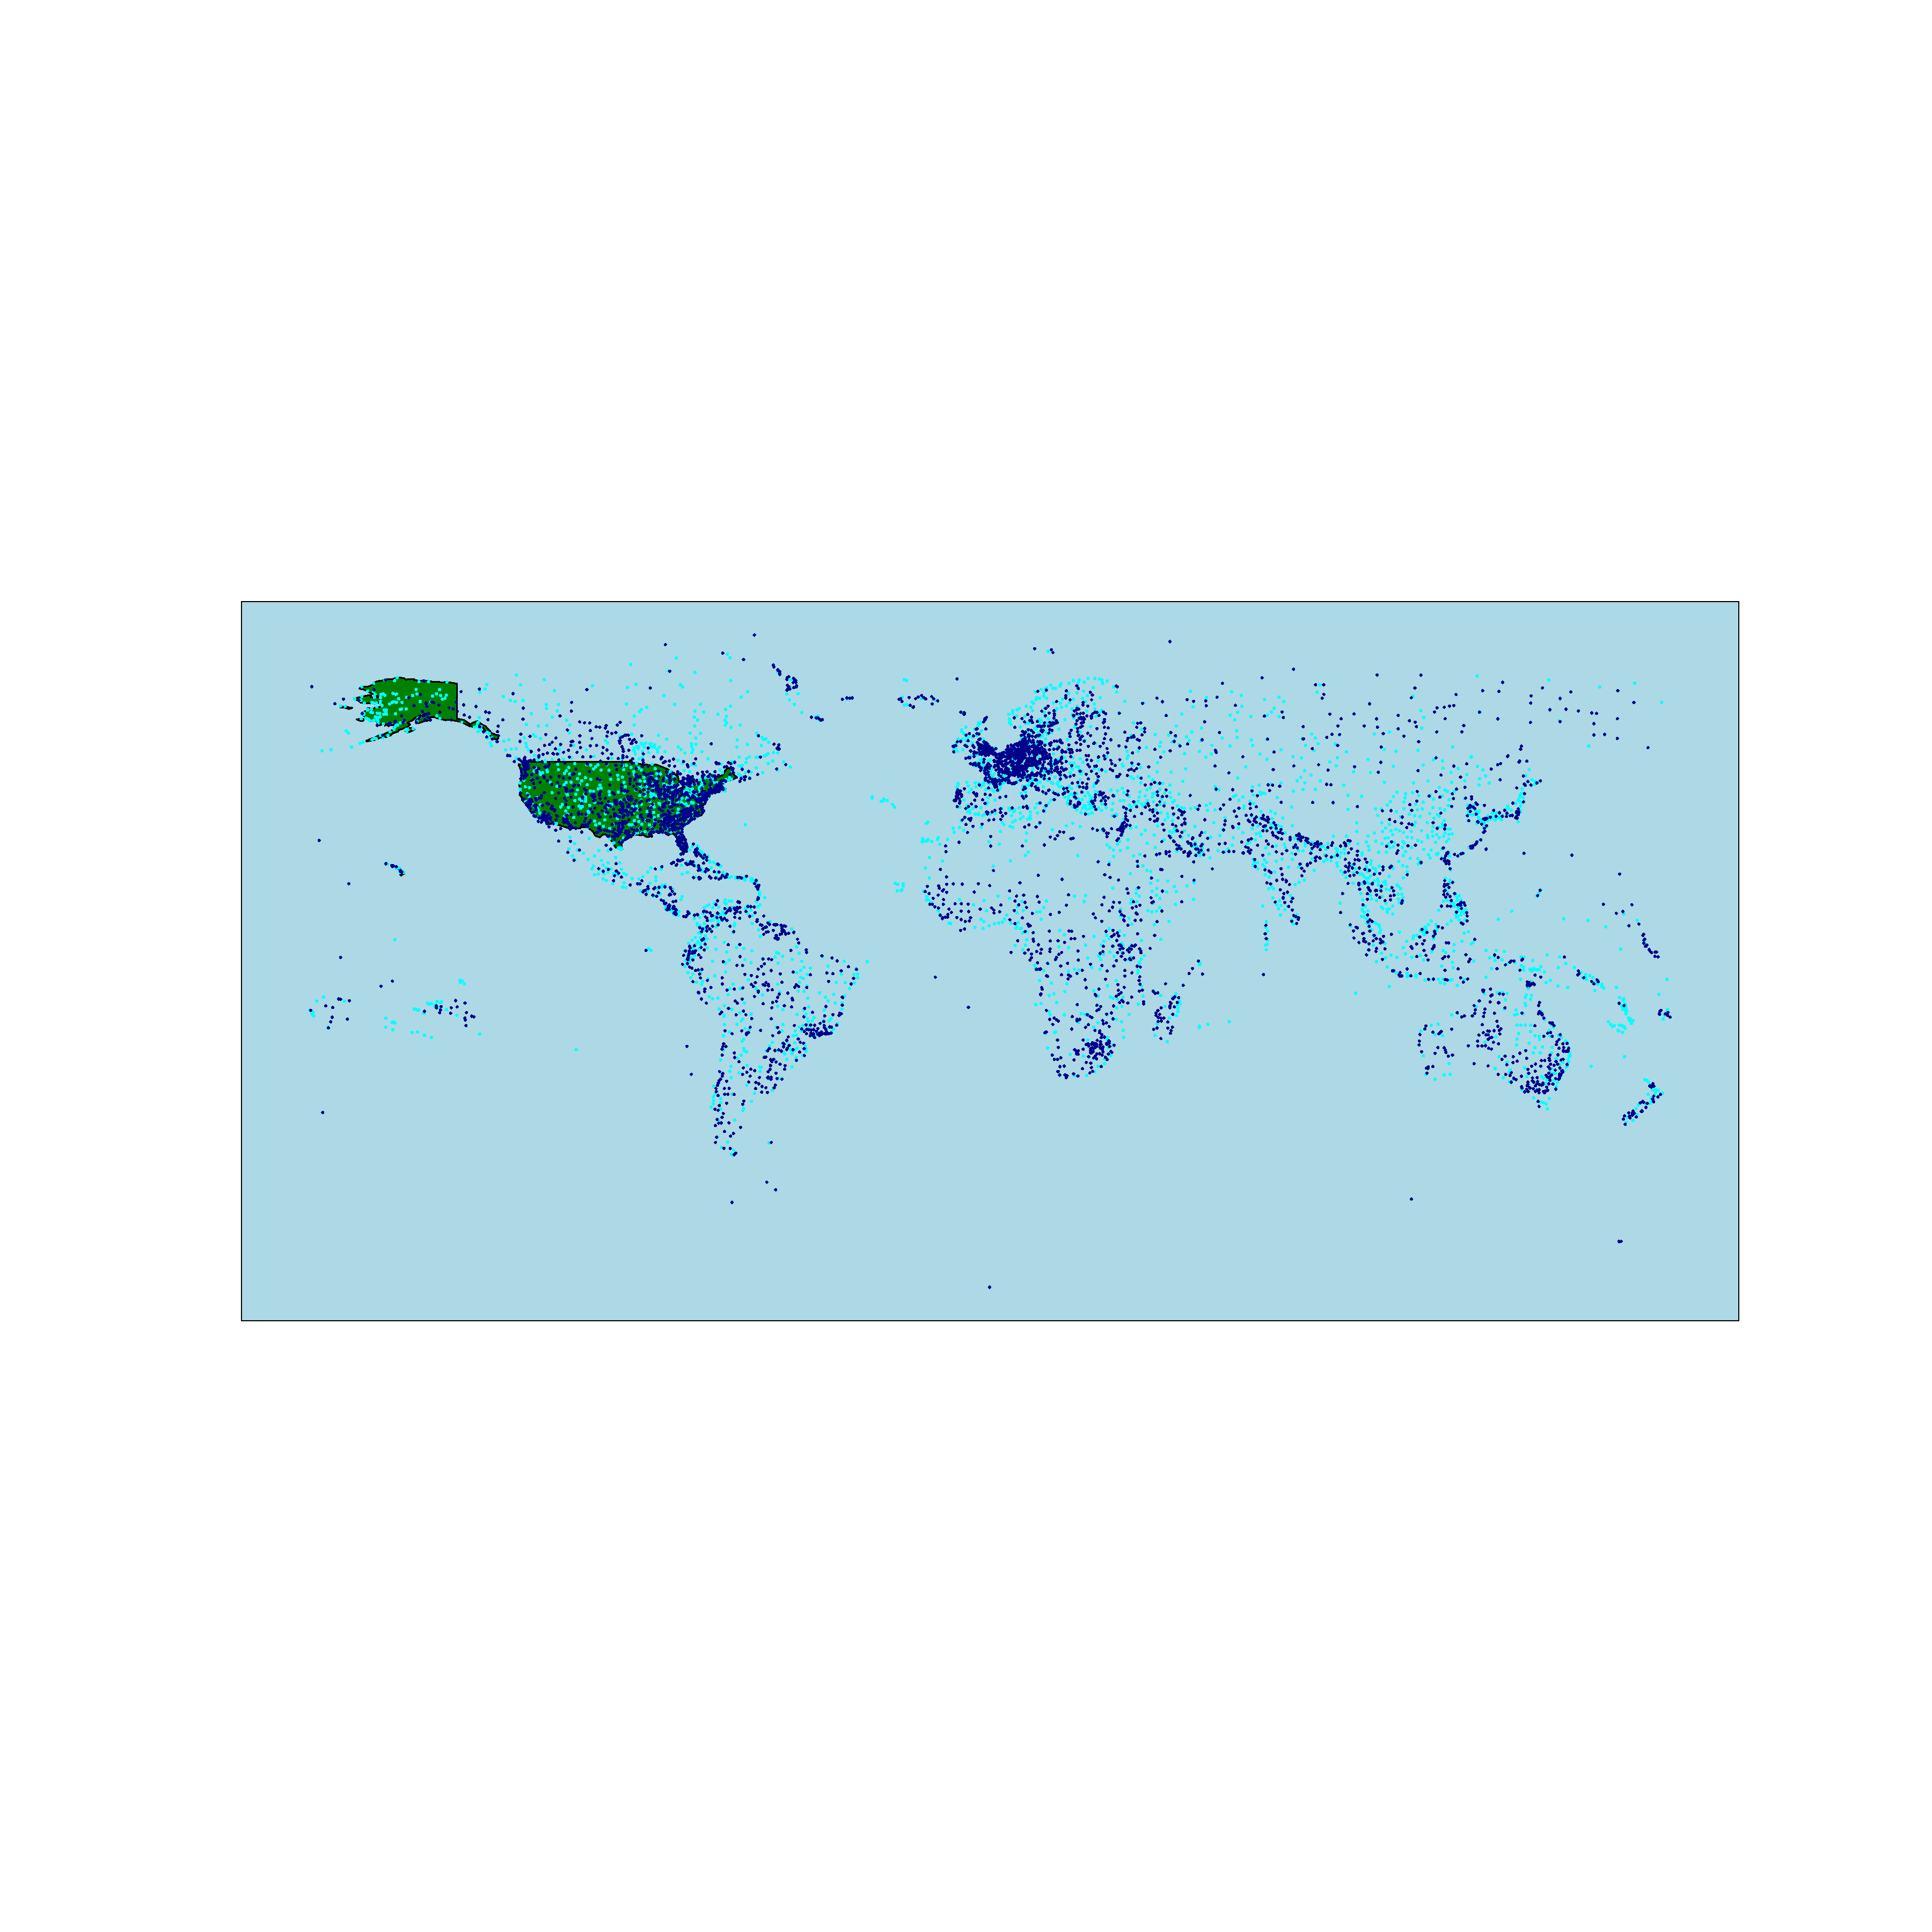
\includegraphics[width=1. \textwidth]{Exam/Airports_WorldMap}
%  \label{fig:airports}
%\end{figure}

\subsection{Price Data}
Price data are scraped from \url{skyscanner.com} using Selenium in Python. Ideally we would have preferred historical prices matching the time horizon of Flight dataset, however we have not be able to find such data. Instead we are scraping prices for all the connections. Due to limited time we have chosen to scrape prices for one specific date. This is problematic since prices shows systematic changes across weekdays, and seasonality across the year. Furthermore, our connection data includes all flight within a year and some routes might not be operated at this particular date.
The scraper function launches a browser and opens the url for a given flight at our chosen date which is May 27th. If possible the price of the cheapest direct flight is chosen. The prices of flights operated by Southwest Airlines are not shown at Skyscanner. If their flight is only one operating, the price of the cheapest indirect flight is chosen. The cheapest indirect flight is also chosen if no carrier is operating at the date.





\section{Empirical Results}
\label{sec:empirical}
% Empirical	Approach
% Description of the empirical model: specification and variables involved
% Strategy for the estimation of the parameters of interest and test of the hypothesis
\subsection{Network Characteristics (T)}
\label{subsec:empirical_network_characteristics}
When analyzing the network we utilize the \texttt{NetworkX} package for Python. We start by characterizing the network. Recall, that we view airports as nodes, and flights between airports as links. Considering the data set of flights in 2018 from the Bureau of Transportation Statistics, we produce a network of US airports and the flights connecting them. We will refer to this network as the US Network. This network has 358 nodes and 3,110 links. Inserting the number of nodes $N$ in equation (\ref{eq:max_links}), the maximum possible number of links would be: 
\begin{align}
    L_{max}  = \frac{358\cdot(358-1)}{2} = 63,903
\end{align}
This implies, that only approximately 5 pct. of possible links are actually found in the network. This sparseness of the network supports the hub-and-spoke view of air transport; rather than having all airports be connected, it is more economically feasible to have certain airports functioning as hubs in their geographical area, and connect to hubs in other regional areas.
\par
Figure \ref{fig:map_general_18} below shows every airport in the network we consider, and the links that connect them. The network is distributed spatially according to the actual geographical locations of the airports, and overlaid on a map of the continental US. From a visual examination the hub-and-spoke nature of the network is clear. Hubs are somewhat distributed geographically and - at a glance - are placed near the larger population centres. Similar maps of the network in 1998 and 2008 can be found in figures \ref{fig:map_general_98} and \ref{fig:map_general_08} in appendix \ref{app:map_general}. The network seems to have been relatively stable over time in the sense that airports that were well connected in 1998 are still well connected in 2018. The business model of a hub-and-spoke structure for the individual airlines is apparent as all of the 15 hubs for the two largest legacy airlines\footnote{Ten hubs of American Airlines, \url{http://news.aa.com/multimedia/default.aspx#factsheets}\\
Eight hubs of Delta Airlines, \url{https://news.delta.com/corporate-stats-and-facts}} are among the large and medium sized hubs, even more so, the network as a whole seem to resemble a hub-and-spoke structure.
\begin{figure}[H]
  \centering
  \caption{Domestic flights network, 2018}
    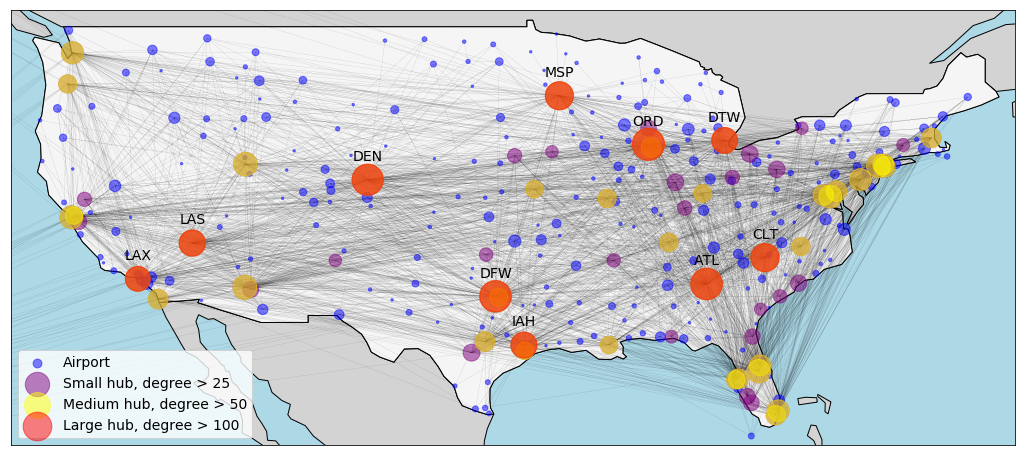
\includegraphics[width=1. \textwidth]{Exam/Figures/map_general_18}
    \vspace{-0.7cm}
    %\notecenter{Size resembles the degree.}
  \label{fig:map_general_18}
\end{figure}
\noindent
To get a further sense of how the network is connected we calculate the \textit{degree centrality} for each node in the network, i.e. the number of other airports each airport is connected to through flights in 2018. The average degree for the 358 airports contained in the data set is 18,0. This average masks a huge variation; the highest degree found in the data is the O'Hare International Airport (ORD) in Chicago with a degree of 176.  Conversely, 51 airports have a degree of 1, implying that in this data set they only appear in connection with a single other airport.
\par
The degree distribution for each of the years 1998, 2008, and 2018 can be seen in figure \ref{fig:degree_distribution} and can also be grasped in figure \ref{fig:map_general_18} through the size and color of the nodes. Clearly, a large number of airports are connected by flights to few other airports, while a minority of airports are much more connected.
\par
Table \ref{tab: temporal} shows key characteristics of the network for 1998, 2008, and 2018 respectively. For the network in 1998, average shortest path length and diameter is not defined, since the network is not connected. The number of airports has risen substantially in the period, as has the number of unique flight routes. The average degree of the network rose from 1998 to 2008, but fell slightly from 2008 to 2018. One should of course keep in mind, that the rise in the number of airports captures both construction of new airports and if existing airports are serviced by airlines that grow and then meet the inclusion criteria for the sample.
\begin{table}[H]
\centering 
\caption{Network Characteristics, 1998-2018}
\label{tab: temporal}
\begin{tabular}{|l|l|l|l|}
\hline
\textbf{}                    & \textbf{1998} & \textbf{2008} & \textbf{2018} \\ \hline
Nodes                        & 209           & 310           & 355           \\
Links                        & 1614          & 2754          & 3110          \\
Average degree               & 15.5         & 18.1         & 17.5          \\
Average shortest path length & -           & 2.33          & 2.39          \\ 
Diameter                     & -             & 5             & 6           \\
Clustering Coefficient       & 0.63          & 0.65          & 0.57          \\ \hline
\end{tabular}
\end{table}
\noindent
To look into an example of how the network structure has changed over time we investigate the network consisting of the small airport Colorado Springs (COS) and its neighbors in figure \ref{fig:map_COS}. In the left panel we see that COS in 1998 was connected to 11 of the 10 closest inland hubs (except for Las Vegas) and only connected to a single airport that is not one of the absolute mayor hubs to an extent where the average degree between the 12 nodes is 10.8 out of possible 11, resulting in a \textit{clustering coefficient} extremely close to unity. This is as close as one could dream of getting to observing a perfect hub-and-spoke network. In order to fly from COS to any West- or East Coast city (or vice versa) it is mandatory to transfer at one of the 10 bigger inland hubs. Interestingly enough, by 2008 several connections to smaller airports were maintained such that the average degree distribution only was 18.4 out of possible 26. This was followed by a reversion such that COS in 2018 again was almost exclusively connected to mayor hubs. The difference being that one now suddenly did not need to transfer to get directly to Florida or New York by the East Coast or to Las Vegas, LA or Seattle by the West Coast. Though the latter two possibly being down to \textit{Frontier Airlines} as mentioned in subsection \ref{subsec:focus_cities}, the process of establishing Colorado Springs as a focus city with important long distance connections clearly did not stop there. However, we should refrain from extrapolating the development of the role of COS to being a general tendency in the network.
\begin{figure}[H]
  \centering
  \caption{Network of Colorado Springs (COS) and its direct neighbors}
    \begin{subfigure}[t]{0.32\textwidth}
        \centering
        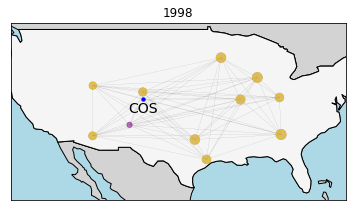
\includegraphics[width=\linewidth]{Exam/Figures/map_COS_98}
    \end{subfigure}
    \hfill
    \begin{subfigure}[t]{0.32\textwidth}
        \centering
        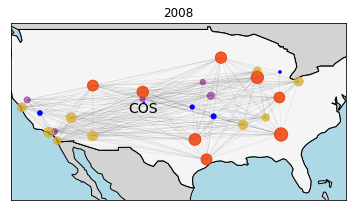
\includegraphics[width=\linewidth]{Exam/Figures/map_COS_08} 
    \end{subfigure}
    \hfill
    \begin{subfigure}[t]{0.32\textwidth}
        \centering
        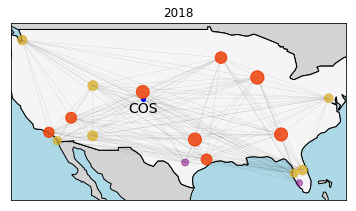
\includegraphics[width=\linewidth]{Exam/Figures/map_COS_18} 
    \end{subfigure}
  \label{fig:map_COS}
\end{figure}
\noindent
The degree distribution of the network is shown in figure \ref{fig:degree_distribution} with a fitted power-law distribution. The hub-and-spoke nature of the network - and the related fact that it is scale-free - is fairly apparent; a large number of nodes have a low degree, while a few nodes have a degree far above the average degree. 
\begin{figure}[H]
  \centering
  \caption{Degree distribution of network, 1998, 2008 and 2018}
    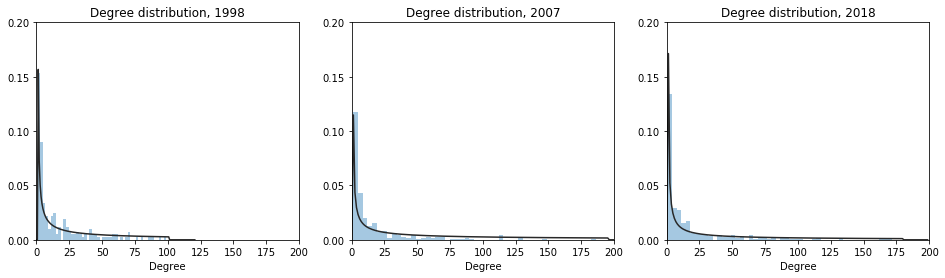
\includegraphics[width=1 \textwidth]{Exam/Figures/degree_distributionv2.png}
  \label{fig:degree_distribution}
\end{figure}
\noindent
As an alternative measures of centrality in the network, we calculate \textit{betweenness centrality} that measures the degree to which an node is part of the shortest path between two other nodes where path length is defined as the number of traversed links.
% Figur med hhv. degree distribution (til venstre) og betweenness centrality (højre)?
\par
An overview of our three key network characteristics, and how they relate, can be seen in figure \ref{fig:Btwns_CC}. First of all, there is a clear positive relationship between degree and betweenness centrality; airports that are linked to a large number of other airports are also more likely to be part of a shortest path between two airports. This is fairly unsurprising. Secondly, there is no simple relationship between clustering coefficient and either of the other measures. A large number of airports have clustering coefficient equal to 1, implying that all their neighbors are connected to each other. There is also a number of airports with a clustering coefficient of 0, implying that none of their neighbors are connected to each other, or that they only connect to one other airport.
\begin{figure}[H]
  \centering
  \caption{Betweenness centrality, clustering coefficient and degree, 2018}
    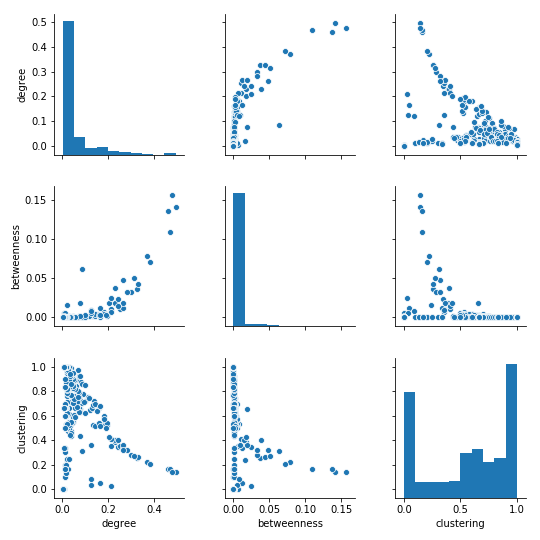
\includegraphics[width=1 \textwidth]{Exam/Figures/NxPairPlot.png}
  \label{fig:Btwns_CC}
\end{figure}
\noindent
In the end, we use clustering coefficient, betweenness and degree as features in the prediction model. Note, that these are all node-specific measures, and as such, for each flight observation, there are two realizations of each measure corresponding to destination and origin airport respectively.

\subsection{Network vulnerability (M)}
We conduct an analysis of how the network is affected when certain nodes are removed. This analysis is broadly in line with the analysis in \cite{chi2004structural}.
\par
Figure \ref{fig:attacks_and_errors} below shows how key network characteristics (average degree, clustering coefficient and global efficiency) are affected, when nodes are removed. One curve corresponds to removal of the most connected nodes, this is what we refer to as an 'attack' on the network, where the hubs are targeted. We likewise consider how the network is affected when we remove the least important nodes first, the occurrence of a so-called 'error'.
\par
%Finally, we consider how the network is affected by an event that removes all network in a geographical area (such as might be the case due to natural disaster and extreme weather conditions). We conduct this analysis by choosing a spot in the continental US, calculating the (geographical) distances from each airport to this spot, and then removing all airports within x miles. This final analysis takes advantage of the spatial nature of the network, and provides insight into how geographically determined failures may affect the network. \\
It should be noted, that in this section we analyze initial consequences for a static network as it is in our data set. Obviously, if a number of airports were to close for a prolonged period (e.g. due to natural disaster), the agents in the market would make changes to the network to accommodate the new situation. Market forces are likely to have been a determinant in producing the network as it is, and exogenous changes to the network would cause changes in behaviour of the agents in the market which would produce a new network.
\begin{figure}[H]
  \centering
  \caption{Effect of node removal on average degree (left) and clustering coefficient (right)}
    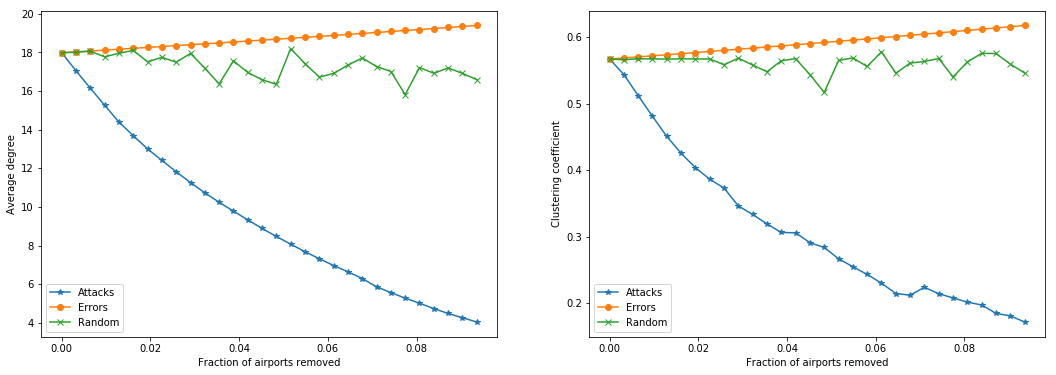
\includegraphics[width=1. \textwidth]{Exam/Figures/attacksanderrors.png}
  \label{fig:attacks_and_errors}
\end{figure}
As figure \ref{fig:attacks_and_errors} shows, the removal of a relatively small number of hubs can dramatically alter network characteristics. Unsurprisingly, removal of the least important nodes increases the measures while. Thus, the network is somewhat vulnerable to 'attacks' on the most connected airports.
\par
In the figure, we also show the effect of removing random nodes. Note, that each point represents a "new" network of randomly chosen nodes in the original network. Nodes left out in the first observation may therefore be present in the second observation. Thus, removal of random nodes has close to no persistent effect on average degree or the clustering coefficient of the network due to mean reversion. This again points to the fact that the network is vulnerable only to a concerted attack on several important hubs.

\subsection{Predicting flight prices - Do network-related features add predictive power? (C)}
We want to assess whether network characteristics can contribute in predicting flight prices compared to a prediction model using only a set of baseline variables. Our set of baseline variables include: The number of flights on the given route in the year considered, the distance between the two airports, the (average) time in minutes for the flight and the number of carriers who flew the route during the year considered, as well as dummies for origin and destination airports. Our set of network-related features includes, for both origin and destination airport: Betweenness centrality, degree and clustering coefficient.
\medskip\\
In order to get a sense of the correlation structures, we show all the continuous variables in the correlation plot in figure \ref{fig:correl}. Unsurprisingly, we see that prices are positively correlated with distance and flight duration and negatively with the number of flights on the route due to competition or economies of scale. We see that the rest of the variables, including all our network variables, are only weakly correlated with prices. It is further seen that some of the features exhibit multicollinearity to some degree.
\begin{figure}[H]
  \centering
  \caption{Correlation Plot}
    
\includegraphics[width=0.9 \textwidth]{Exam/Figures/corr_plot.pdf}
  \label{fig:correl}
\end{figure}
\noindent
In order to predict prices we use a linear prediction model including network characteristics and other things such as distance, flight duration, and airport dummies as predictors. We follow the procedure outline in section \ref{subsec: prediction model}. The procedure is implemented with the \texttt{SKLEARN} python module from which we use \texttt{train\_test\_split}, \texttt{StandardScaler}, \texttt{ElasticNet}, and  \texttt{CVGridSearch}.\footnote{See github for documentation, \url{https://github.com/Morten-Esketveit/TSDS-gruppe-2019}}
\medskip\\
We use a 5-fold cross-validation and for the grid search we allow the L1-ratio to vary between 0.25 and 1, and the alpha parameter to vary between 1 and 20.\footnote{Prior to fitting the model, we scale the features using the \texttt{StandardScaler} in Python. This is done in order to avoid artificially large/small weights which could make convergence difficult when we are using regularization.} Figure \ref{fig:validation curve} plots the score, measured in terms of $R^2$ as a function of the regularization parameter $\alpha$ for the three highest L1 ratios. Using grid search the optimal $\alpha$ is approximately 5.9 %6.2 
whereas the optimal L1 ratio is 1.
\begin{figure}[H]
  \centering
  \caption{Validation Curves}
    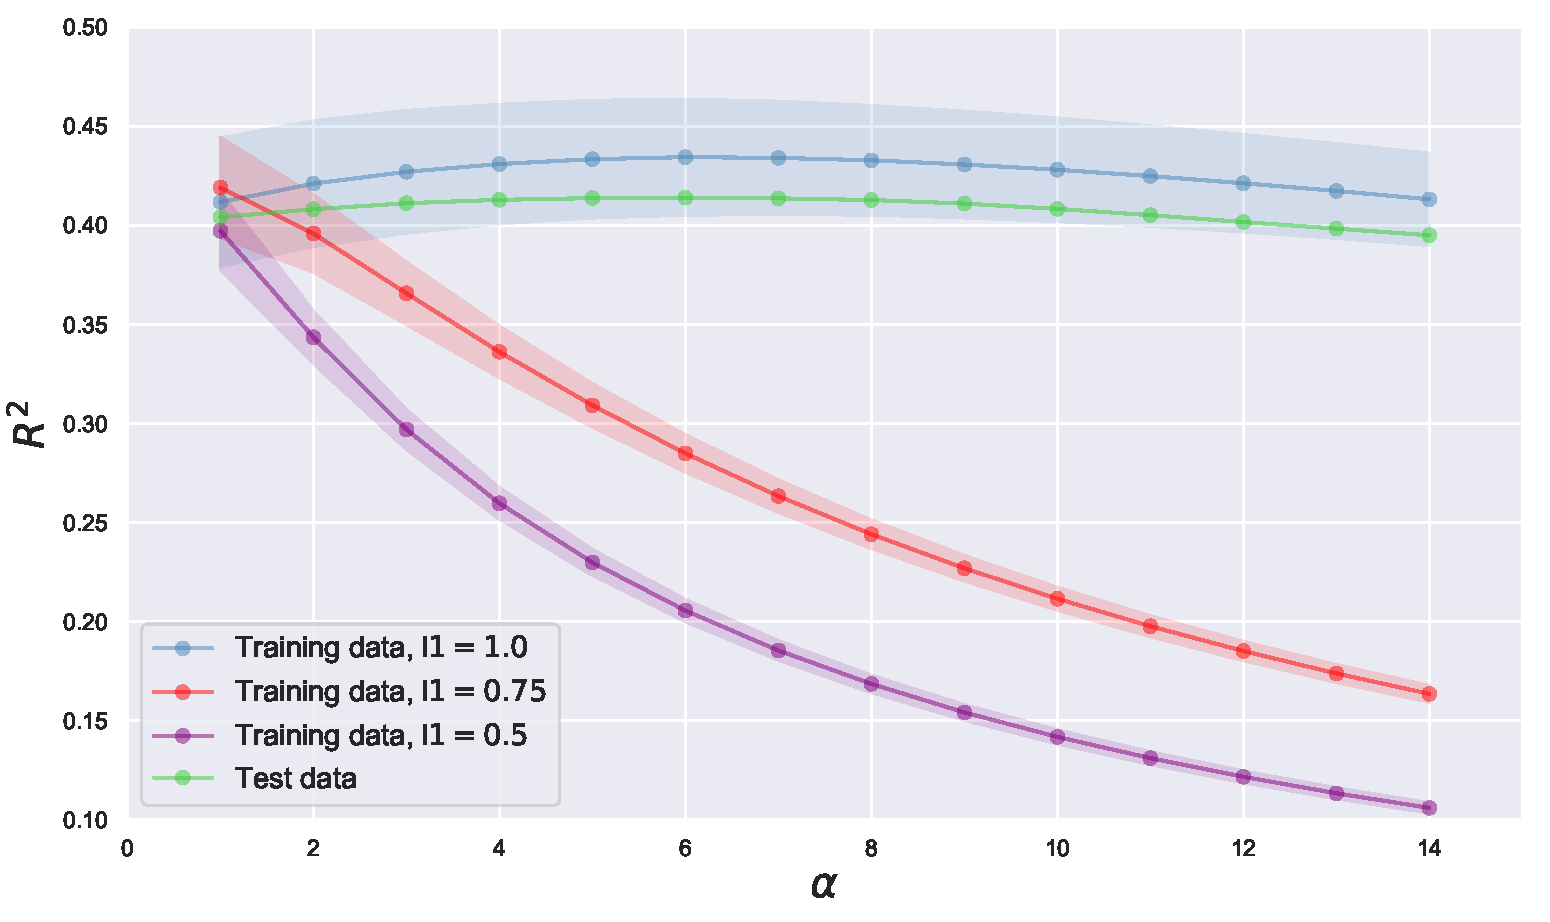
\includegraphics[width=1. \textwidth]{Exam/Figures/validation_curve.pdf}
  \label{fig:validation curve}
\end{figure}
\noindent
Finally, the best model is tested on our test data and the results are compared to the corresponding model without network features. The results are summarized in table \ref{tab: model1}. Our model is able to explain around 40 pct. of the variation in flight prices. We find, that adding network characteristics only increase the out-of-sample prediction marginally, i.e. by 0.5 percentage point. Considering the hyperparametrization both models have a L1 ratio of 1 whereas the $\alpha$ parameter differs slightly. Across the models, the weights of the baseline features are quite similar (see table \ref{tab: coefs} in appendix \ref{app:prediction_model}) for the number of flights, average time, and the number of flights to and from the destination airport. These are the only continuous baseline features with weights that are different from zero. Among the other network features, origin betweenness and both clustering coefficients enters the model with non-zero weights. Based on the size of the coefficients, the clustering coefficient seems to be the most important, however the regularization tends to bias the coefficients. The way the network features enter the model is a result of the correlation structure showed in figure \ref{fig:correl} and the Lasso regularization. Running the model without airport fixed effects (not shown) increases the importance of network characteristics - overall the prediction model performs much worse, however. In this case, the baseline model is able to explain 15.9 percent of the variation whereas the network model can explain 17.9 percent.
\FloatBarrier
\begin{table}[htbp]
  \centering
  \caption{Results, Prediction Model}
  \label{tab: model1}
    \begin{tabular}{rlcccc}
    \hline
          &       & \multicolumn{2}{c}{\textbf{Baseline}} & \multicolumn{2}{c}{\textbf{Networks}} \\ 
          &       & \multicolumn{1}{l}{Test data} & \multicolumn{1}{l}{Training data} & \multicolumn{1}{l}{Test data} & \multicolumn{1}{l}{Training data} \\ \hline
    \multicolumn{1}{l}{Model evaluation} & $R^2$  & \multicolumn{1}{c}{0.421} & \multicolumn{1}{c}{0.427} & \multicolumn{1}{c}{0.426} & \multicolumn{1}{c}{0.431} \\
          &       &  &  \multicolumn{1}{c}{(0.026)}     &       & \multicolumn{1}{c}{(0.028)} \\
    \multicolumn{1}{l}{Hyper parameters} & $\alpha$ & \multicolumn{2}{c}{6.359} & \multicolumn{2}{c}{5.872} \\
          & L1 ratio & \multicolumn{2}{c}{1} & \multicolumn{2}{c}{1} \\ \hline
    \end{tabular}%
  \label{tab:addlabel}%
\end{table}%
\FloatBarrier


\section{Discussion}
\label{sec:results}
% Consequences and implications for the public policy from different expected results.
% Network: vulnerability of network and the missing link to effect on consumers.
Our network analysis is done with data from Bureau of Transport Statistics. While this data set is fairly comprehensive, it does not cover flights by airlines who account for less than one percent of revenues in the sector. The network is therefore not entirely 'complete' insofar as there may be routes or airports only used by airlines that do not appear in the data set.
\medskip\\
The results of our analysis of the domestic US air transport network are broadly consistent with previous results about this network. Firstly, it is a scale-free network, where the majority of airports are linked to relatively few other airports while a few airports are very well connected and act as hubs. A very basic analysis and visual inspection suggests, that the network has become larger over time. Airports tend to keep their `role' over time, although some airports became less well-connected in the period 2008-2018 while others became more well-connected. This may reflect changes `on the ground'; cities and areas that experience e.g. economic growth may attract more flights from a larger number of airports. However, the process of how the network is `generated' and changes over time is beyond the scope of this analysis.
\par
Furthermore, the network is vulnerable to removal of hubs, but tolerant to removal of random nodes. This analysis of the vulnerability of the network is in line with previous academic work. However, it seems to be fairly hard to relate changes in network characteristics (e.g. average degree) for the air transport sector to how customers will actually be affected by a removal of these airports. The economic value of such an analysis is therefore questionable.
\medskip\\
We have taken a fairly basic approach to predicting prices of flights between airports and this is reflected in the fact that we are only able to explain around 40 pct. of the price variation in our test data. There are a number of characteristics of the air transport sector that we do not include in our model, but that may conceivably raise predictive power. Firstly, due to large fixed cost the airport transport sector is characterized by imperfect competition. Airlines are price setters and prices therefore differ from the marginal costs. Whereas the marginal costs are closely linked to flight duration and distance, we have only very limited proxies for demand such as the total number of flight on a given route within a year. In addition, price elasticities for demand are likely to vary across routes and time.
\par
In relation to this, we have considered prices from only one Monday. Airlines tend to exert price discrimination depending on the day of the week. Some flights may have a reduced price on weekdays whereas others may have an increased price depending on whether the flight is considered a `recreational' flight or a `business' flight. 
\par
Moreover, airports are viewed as important infrastructure, and may represent large employers in their geographical area. Therefore, political concerns may cause interventions in the market that may affect prices on specific routes. Even more so, flight prices may also be affected by the types of planes servicing specific routes, and the airlines operating the routes. To incorporate such factors into the model would require a greatly enhanced data set, but would also likely increase the predictive power of our model.
\par
As described in section \ref{sec:background}, the presence of low cost carriers has been shown to affect flight prices. Including a variable to capture this is possible within our data set, but requires a systematic way of demarcating low cost carriers from other airlines. 
Finally, a large number of alternative node or link characteristics exist, some of which may contribute more predictive power in the model than the ones we have chosen. 
\medskip\\
With the above considerations in mind, the relatively poor performance of our prediction model is unsurprising. Our focus has been on investigating whether network characteristics contribute to predictive power. At a basic level, this also means that an attempt to build the best possible predictive model for flight prices has not been the primary focus. While this allows us to evaluate whether including network related characteristics contributes predictive power, it also implies that the conclusions we draw may not generalize. Network related characteristics may add predictive power in our model, but not in a more comprehensive model. This is clear from our analysis; network characteristics are much more important than when when applying a model without airport indicators to capture unobserved heterogeneity.

\section{Conclusion}
\label{sec:conclusion}


\clearpage
\printbibliography
\clearpage

\appendix
\renewcommand\thefigure{\thesection.\arabic{figure}}
\setcounter{figure}{0}
\setcounter{page}{1}
\pagenumbering{roman}

\section{Appendix: Domestic flights network, 1998 and 2007}
\label{app:map_general}
\begin{figure}[H]
  \centering
  \caption{Domestic flights network, 1998}
    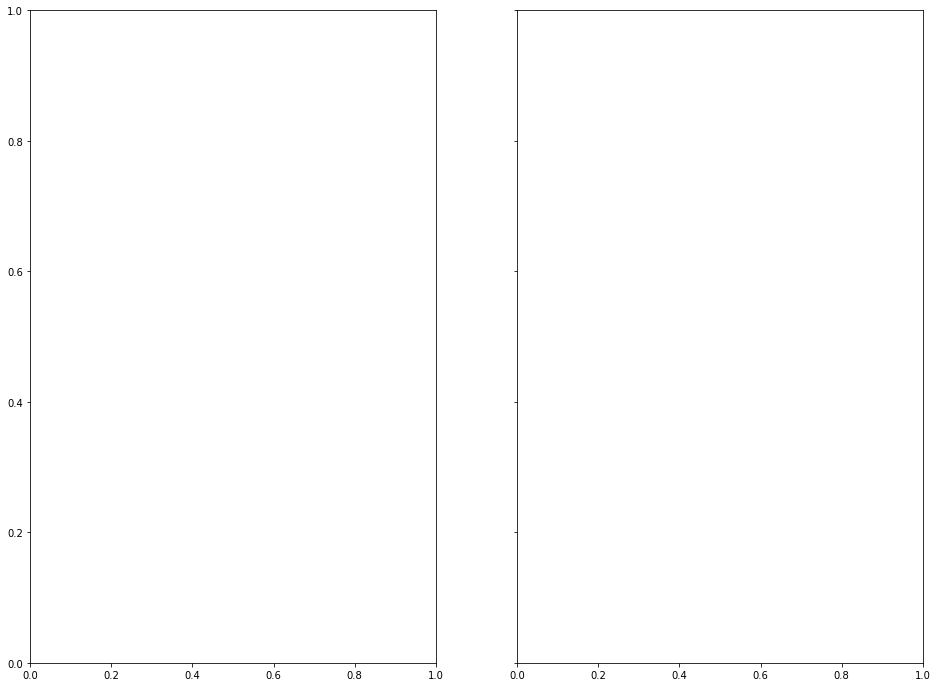
\includegraphics[width=1. \textwidth]{Exam/Figures/map_general_98}
    \vspace{-0.7cm}
    %\notecenter{Size resembles the degree.}
  \label{fig:map_general_98}
\end{figure}

\begin{figure}[H]
  \centering
  \caption{Domestic flights network, 2007}
    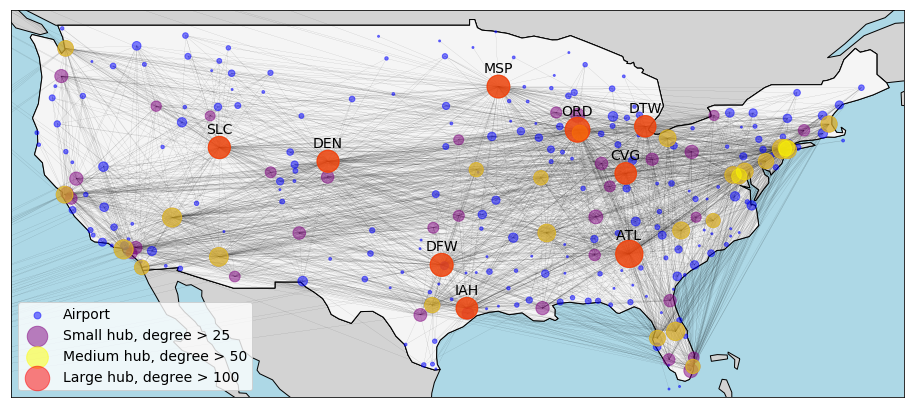
\includegraphics[width=1. \textwidth]{Exam/Figures/map_general_07}
    \vspace{-0.7cm}
    %\notecenter{Size resembles the degree.}
  \label{fig:map_general_07}
\end{figure}

\section{Some other thing}
\label{app:some_other_thing}

\clearpage

\end{document}
